\section{Introduction}

In contemporary AI research, especially as devoted to decision
support, the challenge is often taken to be that of providing AI
support to a single human on their own personal device. However, much
human problem solving is fundamentally social, in that a group of
people must work together to solve a problem, and must rely upon
machine intelligence that is itself highly diverse.  Examples of such
activities include: hiring a person into a university or company,
tackling an emergency crisis like a major water pipeline break,
planning an intricate medical operation, and deciding which companies
to merge with or acquire.  Motivated by such challenges, we are
interested in how an artificial agent --- embedded in a
social-collaboration environment like an immersive room --- can, on
the spot, help a group of human participants.

%%%%%%%%%%%%%%%%%%%%%%%%%%%%%%%%%%%%%%%%%%%%%%%%%%%%%%%%%%%%%%%%%%%%%%
\begin{figure}
\centering
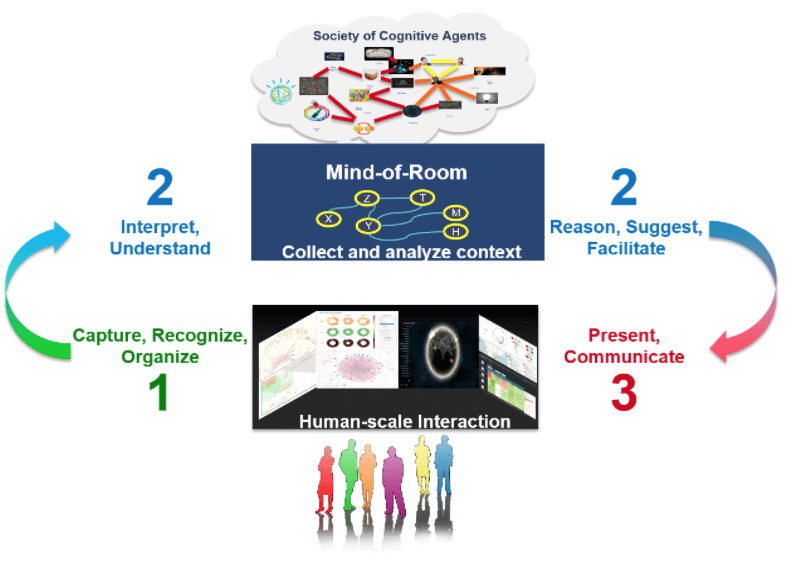
\includegraphics[width=0.5\columnwidth]{chapters/01_introduction/figures/cisl-cycle-graphic.png}
\caption{The flow of information through the elements of a cognitive and immersive system.}
\label{fig:cycle-cais}
\end{figure}
%%%%%%%%%%%%%%%%%%%%%%%%%%%%%%%%%%%%%%%%%%%%%%%%%%%%%%%%%%%%%%%%%%%%%%

We first introduce the notion of a \emph{cognitive and immersive
  system} (CAIS), which comprises three elements linked in a cyclical
flow as shown in Figure \ref{fig:cycle-cais}.  The first element is
responsible for perception and sensing within the environment that
contains the human agents (such as a room). Percepts come courtesy of
a range of sensors, such as microphones and kinects. From these
percepts, we receive information such as what was said, where users
are in the room, etc. The second element, upon receiving that
information, is responsible for interpreting, understanding, and
executing on the basis of that data. In this process, the CAIS may
employ reasoners, planners, databases, etc.\ to drive its
execution. The third element displays both percepts and the results of
processing these percepts in rich, multi-modal ways, such as showing
content on displays or speaking to the users of the system. As part of
the operation of the CAIS, we expect that it has access both to local
modules, as well as is able to make use of external machines and
services that are well-suited to specific tasks or domains. Perhaps
most important to note here is that these external services may be
requested for and opened by users of the system, but that one
reasonably expects that a CAIS should be able to handle these things
in a meaningful and useful fashion.
%% MATT2:  Previous sentence quite hard to understand.  Pls rework.
An important part of our system is that there are overseeing AIs
(agents) operating at the system level that can use the rest of the
system to assist and aid the humans and other AIs that are operating
within.  Thus, the overarching architecture is neither fully
centralized nor fully distributed, but aims to combine the strengths
of both.

Stemming from this overseeing AI, being that it captures all that goes
on within a CAIS, we can look to realize a number of useful
capabilities and principles. Most important here is that these stem
from a rigorous formalization, not from an \textit{ad hoc}
process. From these formal requirements and formalized operations, we
explore how this then also enables our CAIS to possess deeper levels
of understanding of human agents within the room, operating at a
proper theory-of-mind level~\cite{premack_does_1978}, and makes
capable automated means of reasoning, planning, and plan recognition.
An example of this is shown in the following section, and further
explored in Chapter~\ref{chap:planning}, utilizing reasoning to
determine the knowledge and belief of agents, and plan recognition of
what agents are attempting to accomplish to provide meaningful
assistance.

This dissertation is divided into three major parts. The first part
consists of this chapter and deals with the high level goals we lay
out for cognitive-and-immersive systems. We present a motivating
example, and discuss at a high-level abstract view what an idealized
CAIS may be able to accomplish. The second part of the dissertation
concerns mplementation of a real-world CAIS, focusing on two novel
compoments that allow us to to achieve mechanisms being multi-modal
and multi-user without having the system then be constrained to one
specific type of use case or domain. This part is encapsulated in
Chapters 2, 3, and 4. For the third part, which makes up Chapters 5
and 6, we now provide a formalization for these sorts of systems,
stemming from the implmentation in part 2, and then look to see how we
can utilize this for tasks in reasoning, planning, and plan
recognition. Finally, we conclude the work with a summary of our
contributions and recognize promising avenues of future work that
exist.
